\documentclass[red]{beamer}
\mode<presentation>

\usepackage{graphicx}
\usetheme{Warsaw}
\useoutertheme[subsection=false]{smoothbars}

\title{Accelerating the Astronomical Source Finding Process} 

\author{Yaseen Hamdulay and Jarred de Beer}
\institute{{\tiny supervised by} Michelle Kuttel and Sarah Blythe}
\date{26 May 2015}

\begin{document}
\frame{
    \titlepage
}

\section[Outline]{}
\frame{\tableofcontents}

\frame{\frametitle{Survey Example: Noisy}
\centering 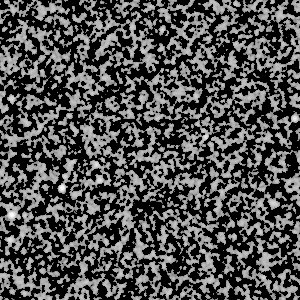
\includegraphics[scale=.75]{noisenoisegalaxy}
}

\frame{\frametitle{Survey Example: Denoised}
\centering 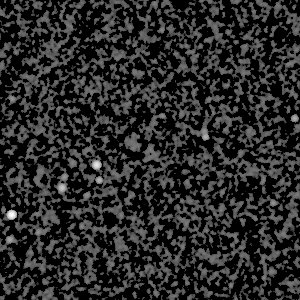
\includegraphics[scale=.75]{noisenoisenoisegalaxy}
}

\section{Introduction}
\subsection{Source Finding}
\frame{\frametitle{What is Radio Astronomy Source Finding?}
\begin{itemize}
\item Process of identifying galaxies or other objects from blind surveys
of the sky. 
\item It is made difficult by the amount of noise that gets detected.
\item Traditionally done by astronomers by hand. 
\end{itemize}
}

\frame{\frametitle{Automated Source Finders}
\begin{itemize}
\item Source finders perform differently with respect to completeness and reliability as they often trade one off for the other.
\item \textbf{Reliability} is the ratio of true positive detected sources to total sources.
\item \textbf{Completeness} is the ratio of sources detected to actual sources.
\item It is useful to have a variety of source finders depending on an astronomers work load. 
\item Accelerating two source finders: DUCHAMP and SoFiA's Source and Clip finder.
%We intend to work on two source finders independently. This prevents either of us from blocking the other.
\end{itemize}
}


\subsection{Research Questions}
\frame{\frametitle{Research Questions}
\textbf{Yaseen:} Can a GPU implementation of the A'trous Wavelet Reconstruction algorithm accelerate the 
DUCHAMP source finding process and how much speedup can be obtained?

\textbf{Jarred:} Can a GPU implementation of the S+C algorithm accelerate the SoFiA source finding process
and how much speedup can be obtained?
}

\subsection{GPU}
\frame{\frametitle{GPU}
\begin{itemize}
\item GPU's are low-cost highly parallel coprocessors. 
\item Difficult to program on due to highly parallel nature and unusual memory hierarchy
\end{itemize}
}

\frame{\frametitle{Automated Methods}
\begin{itemize}
%It is clear that we need automated methods of source finding.
\item There exist automated source finders with DUCHAMP being the
most well known. 

\item With the next generation of Radio Interferometers we are
expecting current generation source finders to take between
hours and days.

\item We are proposing to use GPU's to accelerate the source finding process.
\end{itemize}
}


\section{Work Distribution}
\frame{
    \begin{enumerate}
    \item Implement single-threaded version of algorithm.
    \item Correctness check.
    \item Implement naive version of algorith on GPU.
    \item Correctness check and performance comparison.
    \item Accelerate.
    \end{enumerate}
}

\section{Source Finders}
\subsection{Yaseen (DUCHAMP)}
\frame{\frametitle{Yaseen, DUCHAMP}
\begin{itemize}
\item DUCHAMP is a complete source finding package that is well-known in the astronomy community
\item According to Popping et al DUCHAMP performs the best in terms of completeness and reliability
for point sources and one of the best for larger galaxies which makes it a good target for acceleration. 
\end{itemize}
}

\frame{\frametitle{Pipeline overview}
\begin{figure}
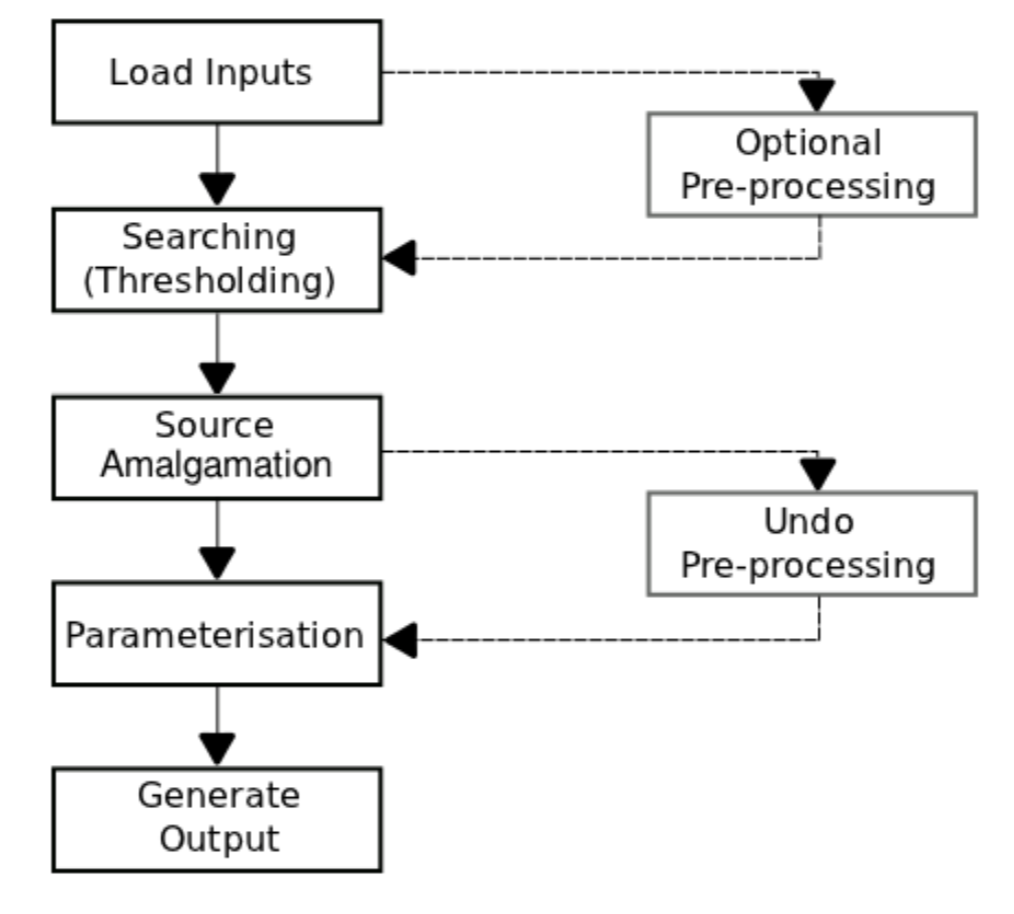
\includegraphics[scale=.3]{duchamp-pipeline}
\caption{DUCHAMP pipeline}
\end{figure}
The DUCHAMP package takes a data cube and pushes it through a pipeline
with data cube at one end and the parameterised sources at the other.

% load inputs 
%   load data cube from a FITS file. 
% pre-processing
%   a'trous algorithm wavelet reconstruction, removes noise
% searching
%   1. signal to noise ratio (some standard deviation's are flagged)
%   2. simple threshold
%   3. false disvoery rate

% source amalgamation
%  taking adjacent detected voxels and merging them together (merging O(N^2))




% wavelet reconstruction up to 92% of run time
% a'trous wavelet reconstruction is essential to DUCHAMP's performance
}

\frame{\frametitle{Preprocessing}
% a'trous wavelet reconstruction
%  convolves with multiple filter banks at different resolutions
% slow due to inefficient memory access patterns. GPU's are good at this (shared memory)
%  
\begin{itemize}
\item Between 65\% and 92\% of the source finding time.
\item DUCHAMP uses the A'trous wavelet reconstruction algorithm.
\end{itemize}

% lower bound of 65% of total run time for data cubes populated with sources when the merging O(N^2) algorithm takes over
% upper bound of 95% of total time 
}

\frame{\frametitle{A'trous Wavelet Reconstruction}
\begin{figure}
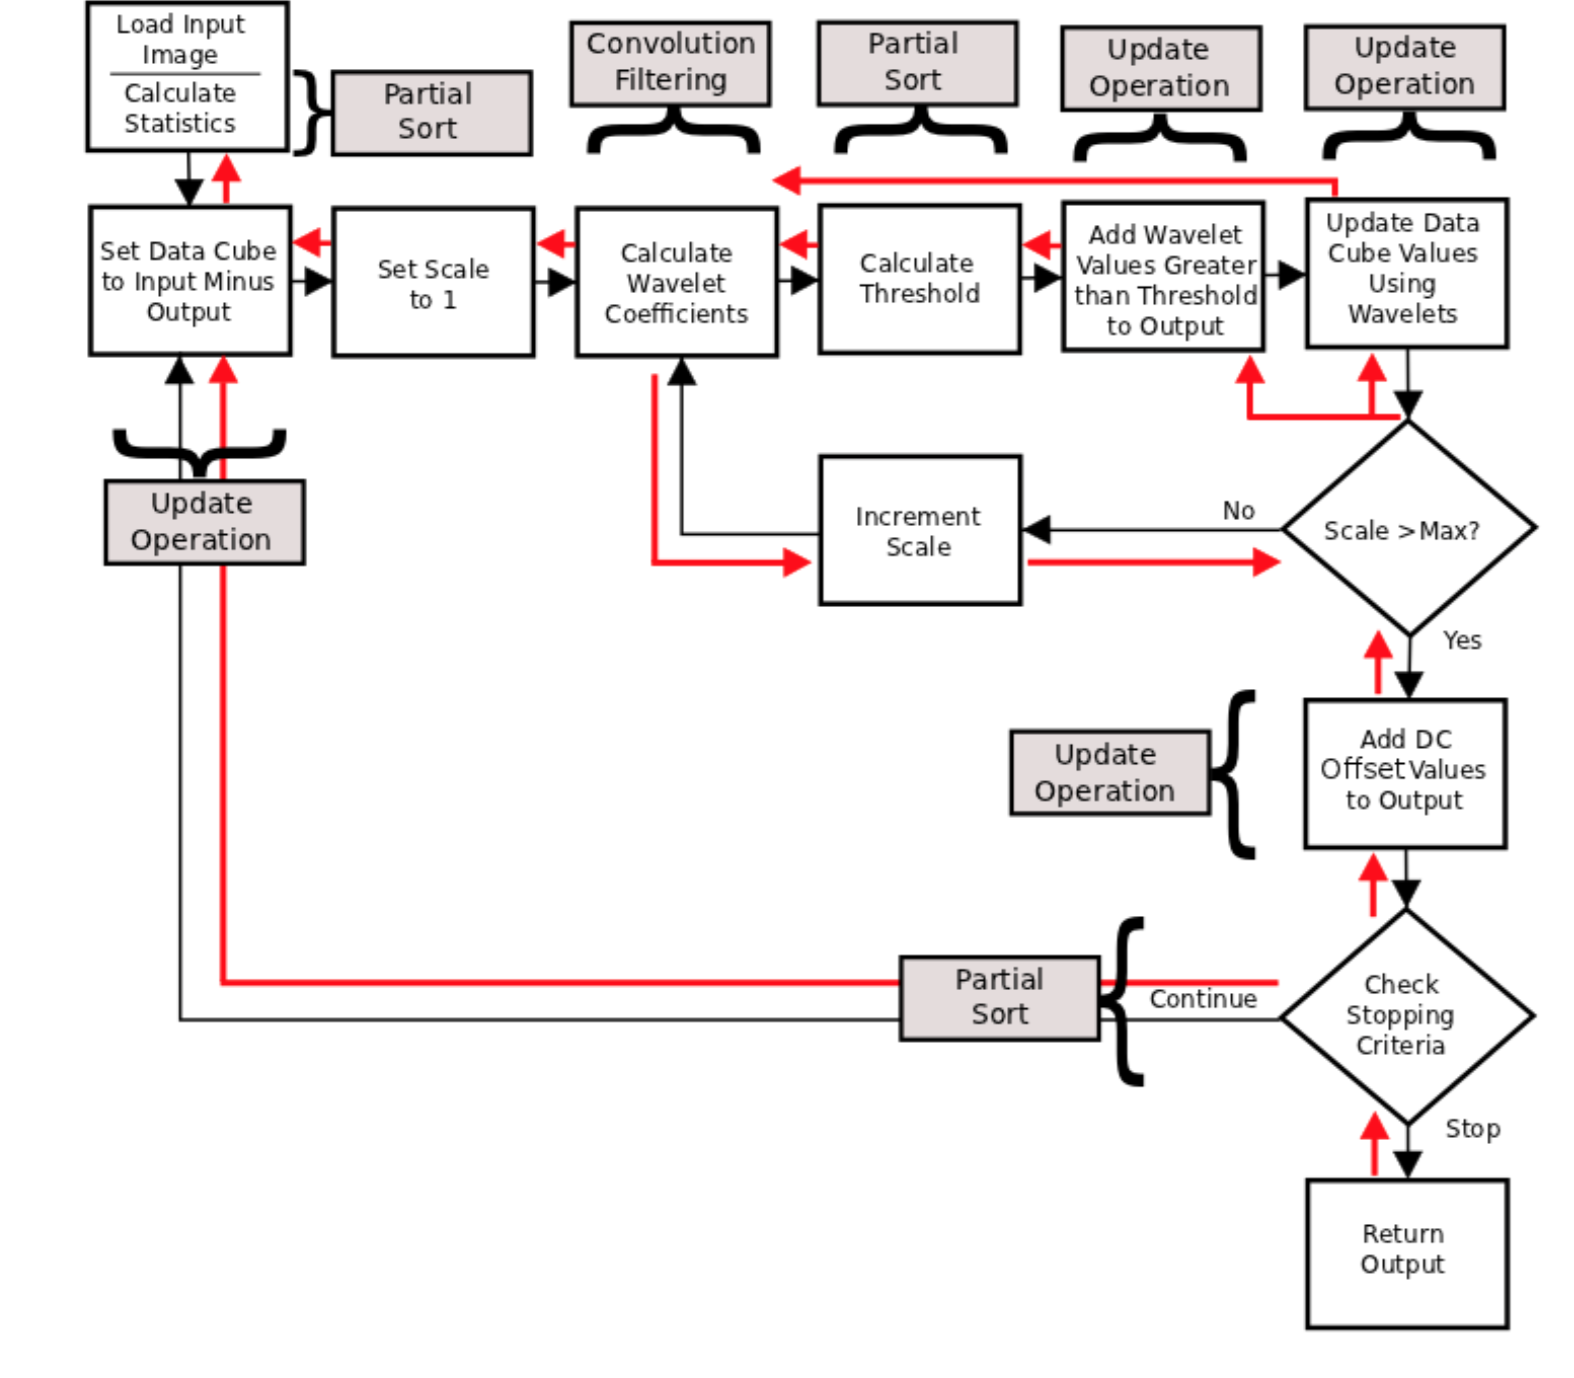
\includegraphics[scale=.3]{atrous}
\caption{Overview of the A'trous algorithm}
\end{figure}
% it's pretty complicated, i won't go through the details
}

\frame{\frametitle{If we have enough time}
    The merging algorithm is in $O(N^2)$, for data cubes with many sources this
    can quickly take lots of time. Implementing on GPU can potentially speed this up.
}

\subsection{Jarred (SoFia, Smooth and Clip Filter)}

\frame{\frametitle{Jarred, SoFia: Smooth and Clip filter}
}

\frame{\frametitle{SoFiA}
    \begin{itemize}
        \item Developed for use on various ASKAP surveys
        \item Designed to be general purpose
        \item Modular and extensible
        \item User specifies which parameters and algorithms to be run
        \item Available on Github, released GPLv3
    \end{itemize}
}

\frame{\frametitle{SoFiA pipeline}
    \begin{figure}
        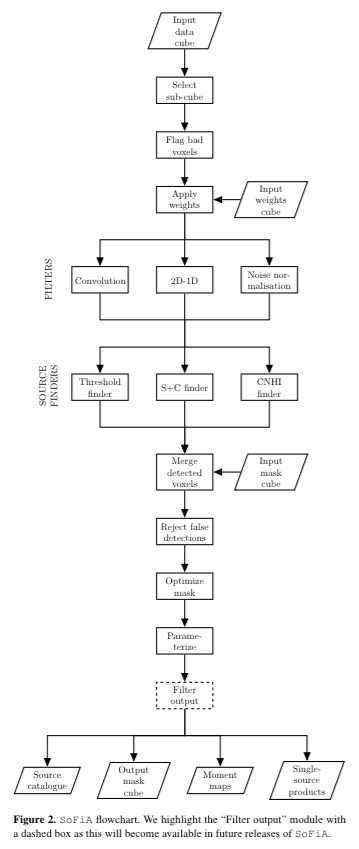
\includegraphics[scale=.3]{sofia-pipeline}
        \caption{DUCHAMP pipeline}
    \end{figure}
}

\frame{\frametitle{Smooth and Clip}
    \begin{itemize}
        \item Developed by Serra et al. (2012)
        \item Searches for emission at multiple frequency resolutions
        \item User specifies the 3D kernels to use
        \item For example:\\
            Smooth the sky with a Gaussian filter\\
            Smooth the velocity separately with a box filter of 2, 4, 8, 16, and 32 channels.
        \item Create a mask for each filter with voxels above an absolute threshold
        \item Final mask is union of all masks
    \end{itemize}
}

\section{Related Work}
\frame{\frametitle{Related Work}
\begin{itemize}
\item Selavy, CPU parallel implementation of DUCHAMP.
\item Badenhorst et al also did a CPU parallel implementation of the wavelet reconstruction filtering algorithm.
\item Gary Resnick, a previous honours student, accelerated the searching (thresholding) part of the source finder. 
\item Parallel Gaussian Source Finder noise suppression has been ported to the GPU with massive performance improvements.

\end{itemize}
}

\section{Evaluation}
\frame{\frametitle{Evaluation}
\begin{itemize}
\item The primary goal of this project is to accelerate the source finding
process. Our most important metric is therefore execution speed.
\item The execution time of the overall source finder depends on the data
cube it is executing on. We should keep this constant or use predetermined
data cubes.
\item Compare against single threaded implementation.
\item Ensuring correctness is of utmost importance.
\end{itemize}
}

\end{document}
